\documentclass[a4paper, 11pt]{article}
\usepackage{comment} % enables the use of multi-line comments (\ifx \fi)
\usepackage{lipsum} %This package just generates Lorem Ipsum filler text.
\usepackage{fullpage} % changes the margin
\usepackage[brazilian]{babel}
\usepackage[utf8]{inputenc}
\usepackage[T1]{fontenc}
\usepackage{graphicx}
\usepackage{indentfirst}
\usepackage[table]{xcolor}

\begin{document}
\noindent
\large\textbf{Melhoria de Processo de Software / Terceiro trabalho}\\
Lucas Albuquerque Medeiros de Moura \hfill 11/0015568 \\
Luciano Prestes Cavalcanti \hfill 11/0035208

\section*{Relatório Avaliação de Processo}

Este relatório visa descrever os resultados encontrados no processo de
desenvolvimento descrito no segundo trabalho da disciplina de Melhoria de
Processo de Software. O relatório irá abranger então uma breve descrição do
processo a ser analisado e seu contexto juntamente com a avaliação e melhoria
desse processo.

\section*{Processo Escolhido}

O processo escolhido para receber a avaliação foi o processo usado pelo
Laboratório Avançado de Pesquisa e Produção de Software (LAPPIS) para o
desenvolvimento do software \textit{Noosfero}. Tal processo pode ser visto na
figura \ref{fig:processo_noosfero}

\begin{figure}[h]
  \centering
  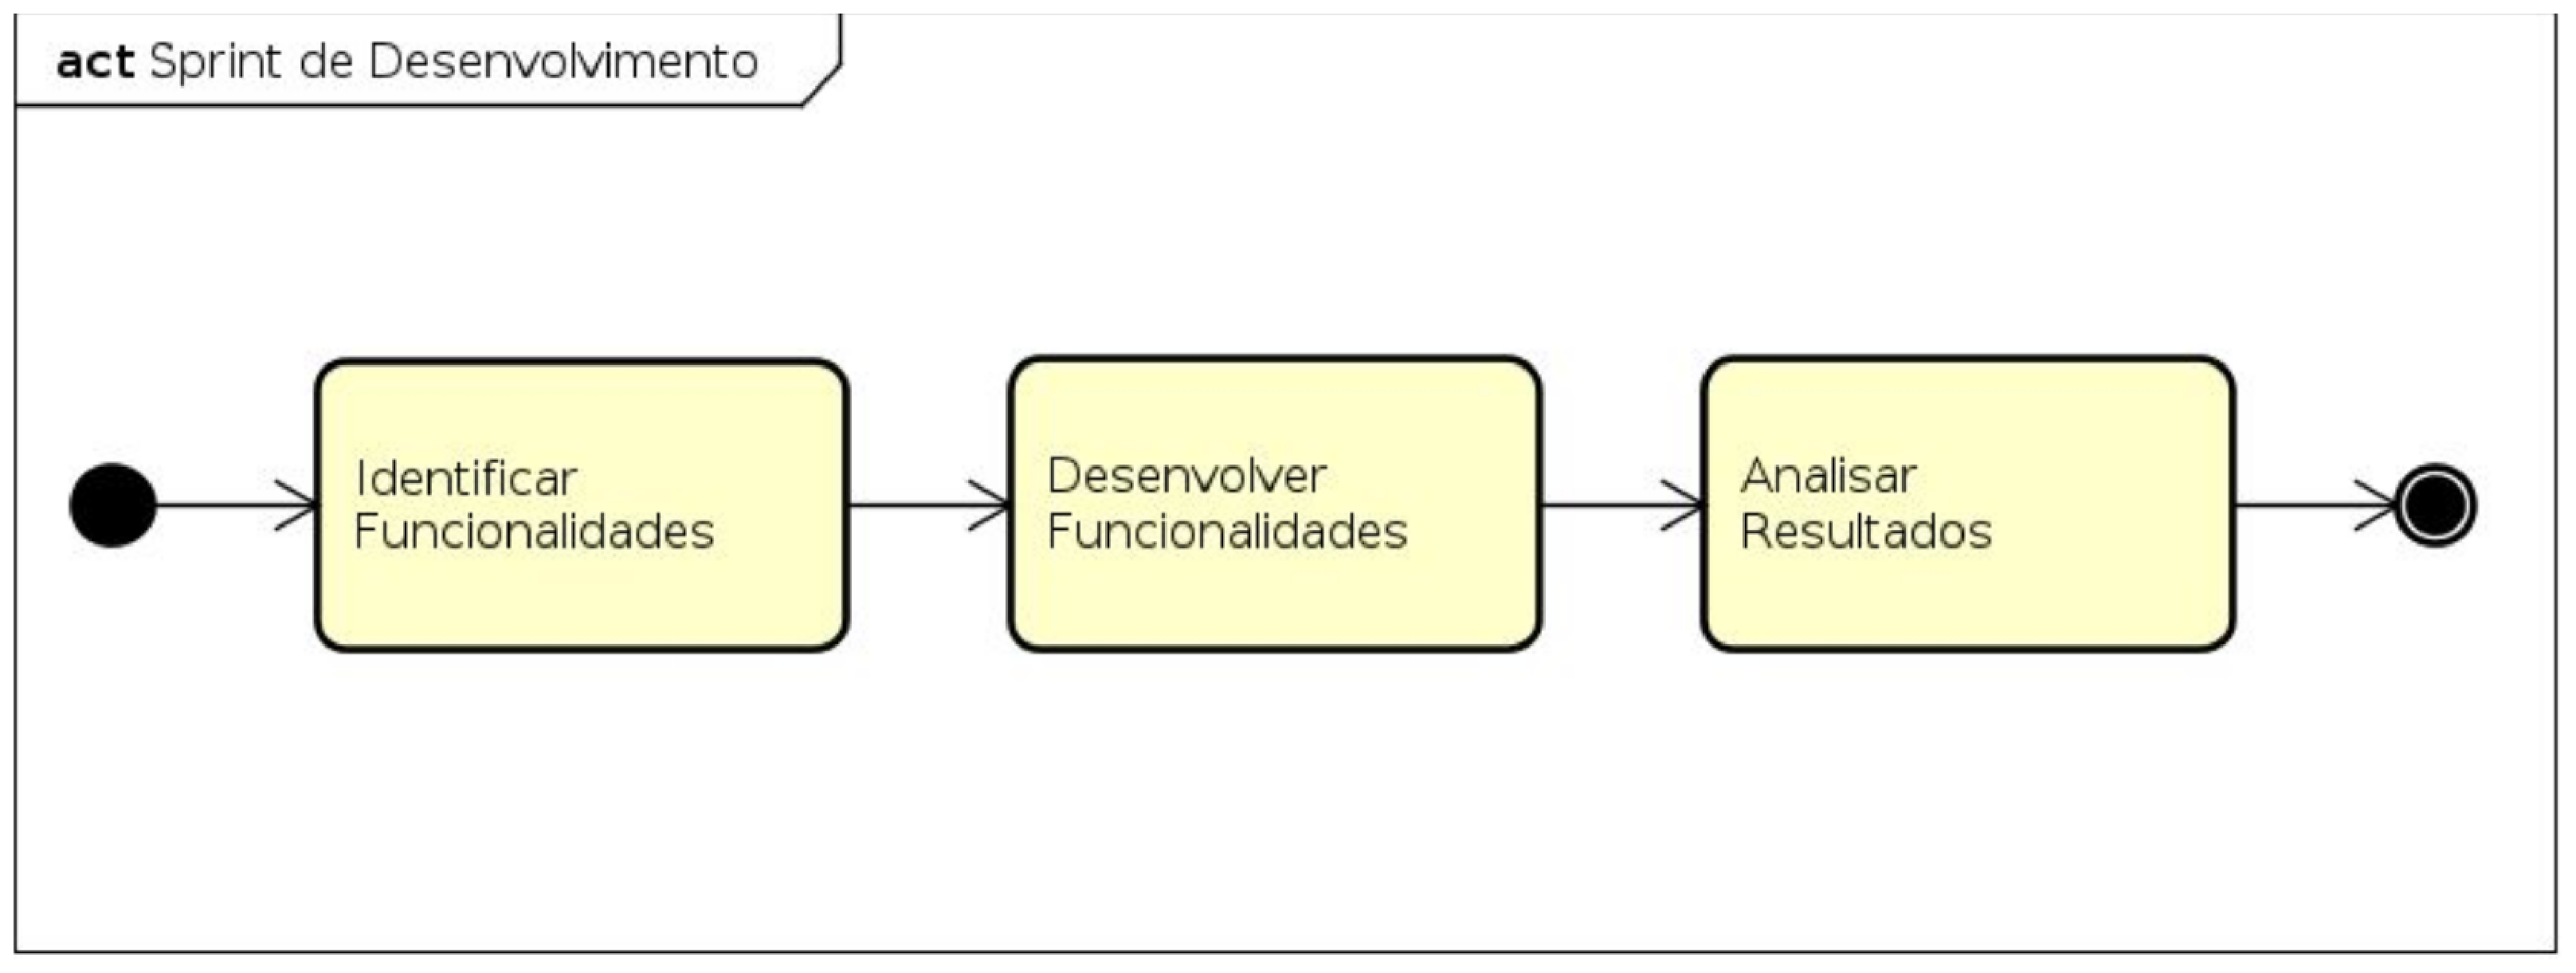
\includegraphics[width=0.9\textwidth]{figuras/processo_mps.eps}
  \caption{Processo de desenvolvimento para o software Noosfero}
  \label{fig:processo_noosfero}
\end{figure}

Tal processo é dividido em três fases distintas, sendo a primeira a fase de
identificar as funcionalidades. Tal fase tem como objetivo definir com a equipe
e o cliente o que será realizado durante uma \textit{sprint}. O processo para
essa fase pode ser visto na figura \ref{fig:processo_noosfero_funcionalidade}

\begin{figure}[h]
  \centering
  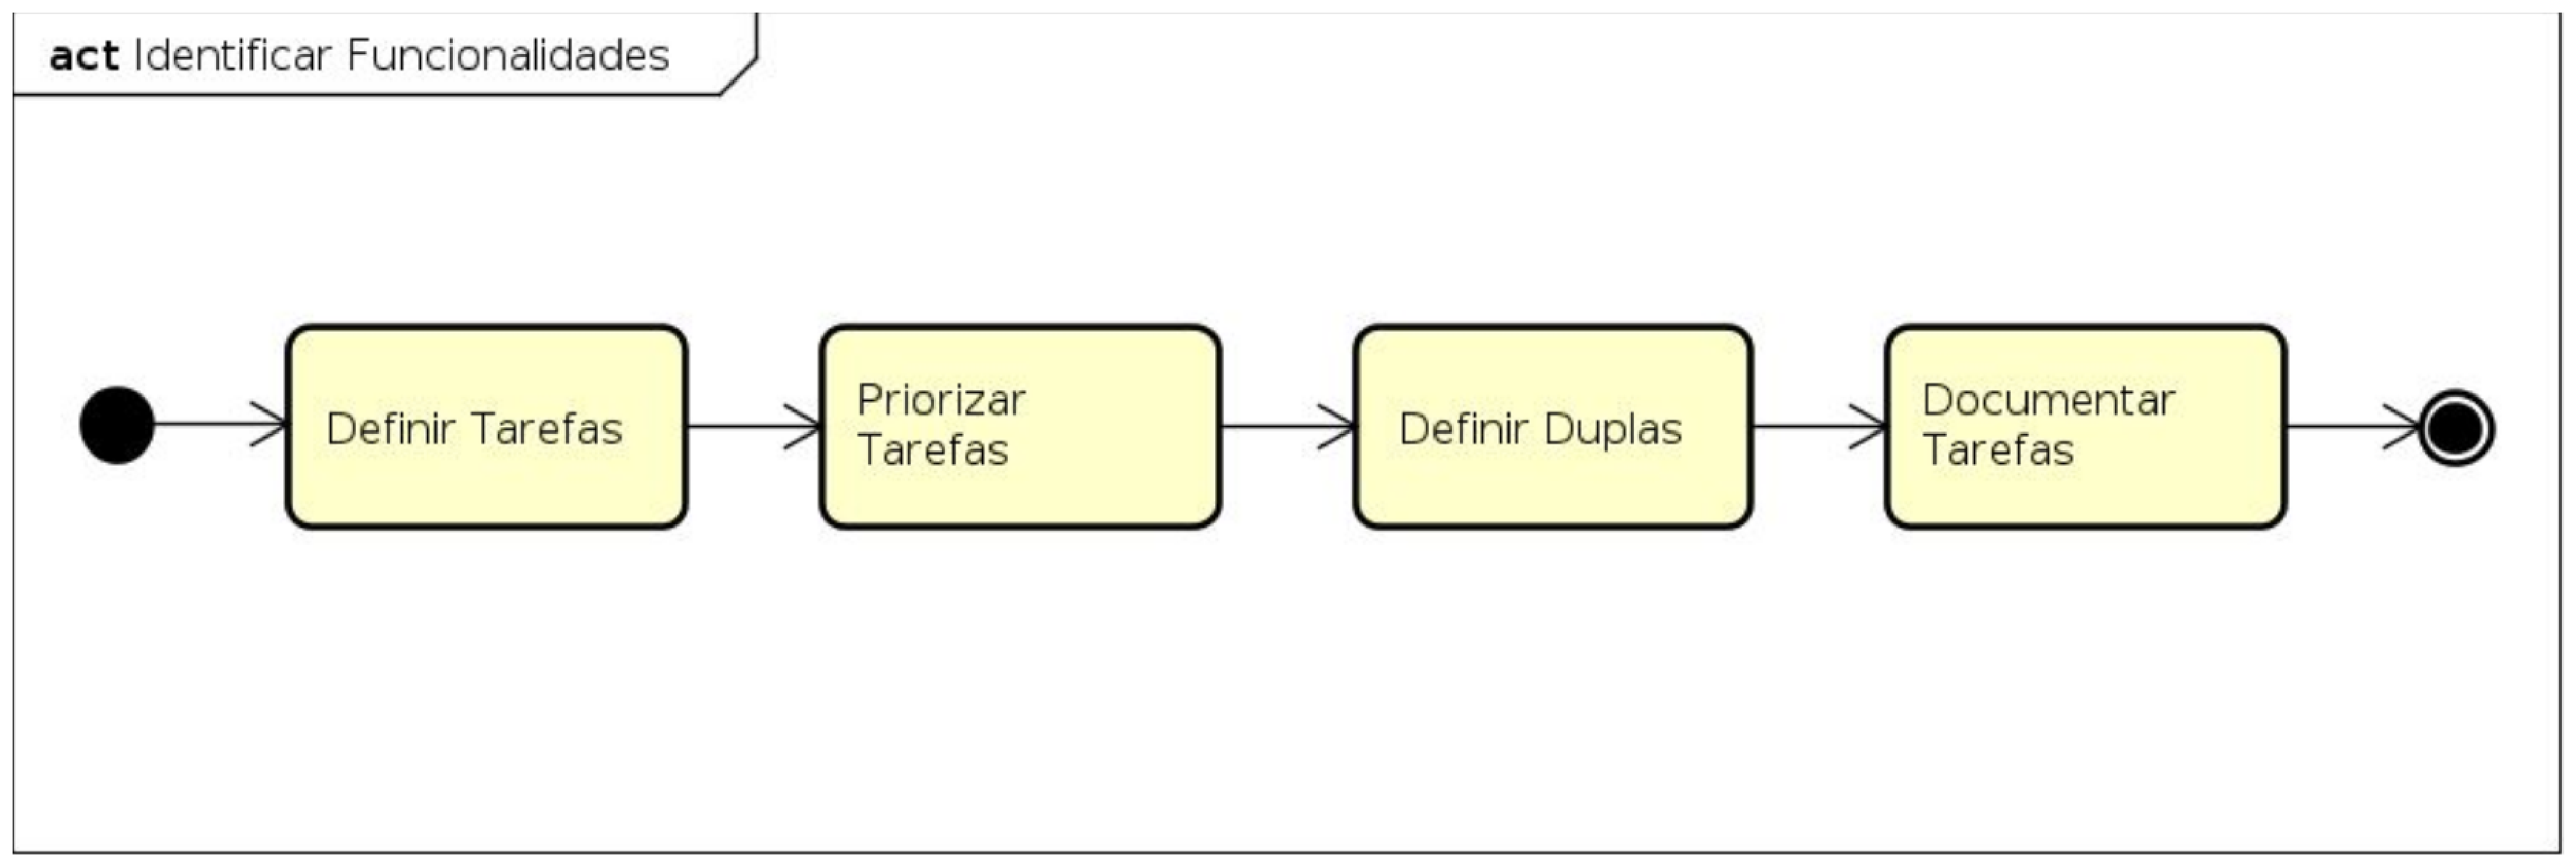
\includegraphics[width=0.9\textwidth]{figuras/processo_mps_funcionalidades.eps}
  \caption{Processo de identificar funcionalidades para o software Noosfero}
  \label{fig:processo_noosfero_funcionalidade}
\end{figure}

A segunda fase do processo é a desenvolver as funcionalides descritas na
primeira fase. As atividades de tal fase do processo podem ser vistas na figura
\ref{fig:processo_noosfero_desenvolvimento}

\begin{figure}[h]
  \centering
  \includegraphics[width=0.9\textwidth]{figuras/processo_mps_desenvolvimento.eps}
  \caption{Processo de desenvolver funcionalidades para o software Noosfero}
  \label{fig:processo_noosfero_desenvolvimento}
\end{figure}

Por fim, a última etapa do processo é a de reportar os resultados da sprint,
tanto em questão do que foi desenvolvido tanto sobre o que o time precisa
melhorar ou focar para próxima sprint. As atividades dessa fase do processo
podem ser vistas na figura \ref{fig:processo_noosfero_resultado}

\begin{figure}[h]
  \centering
  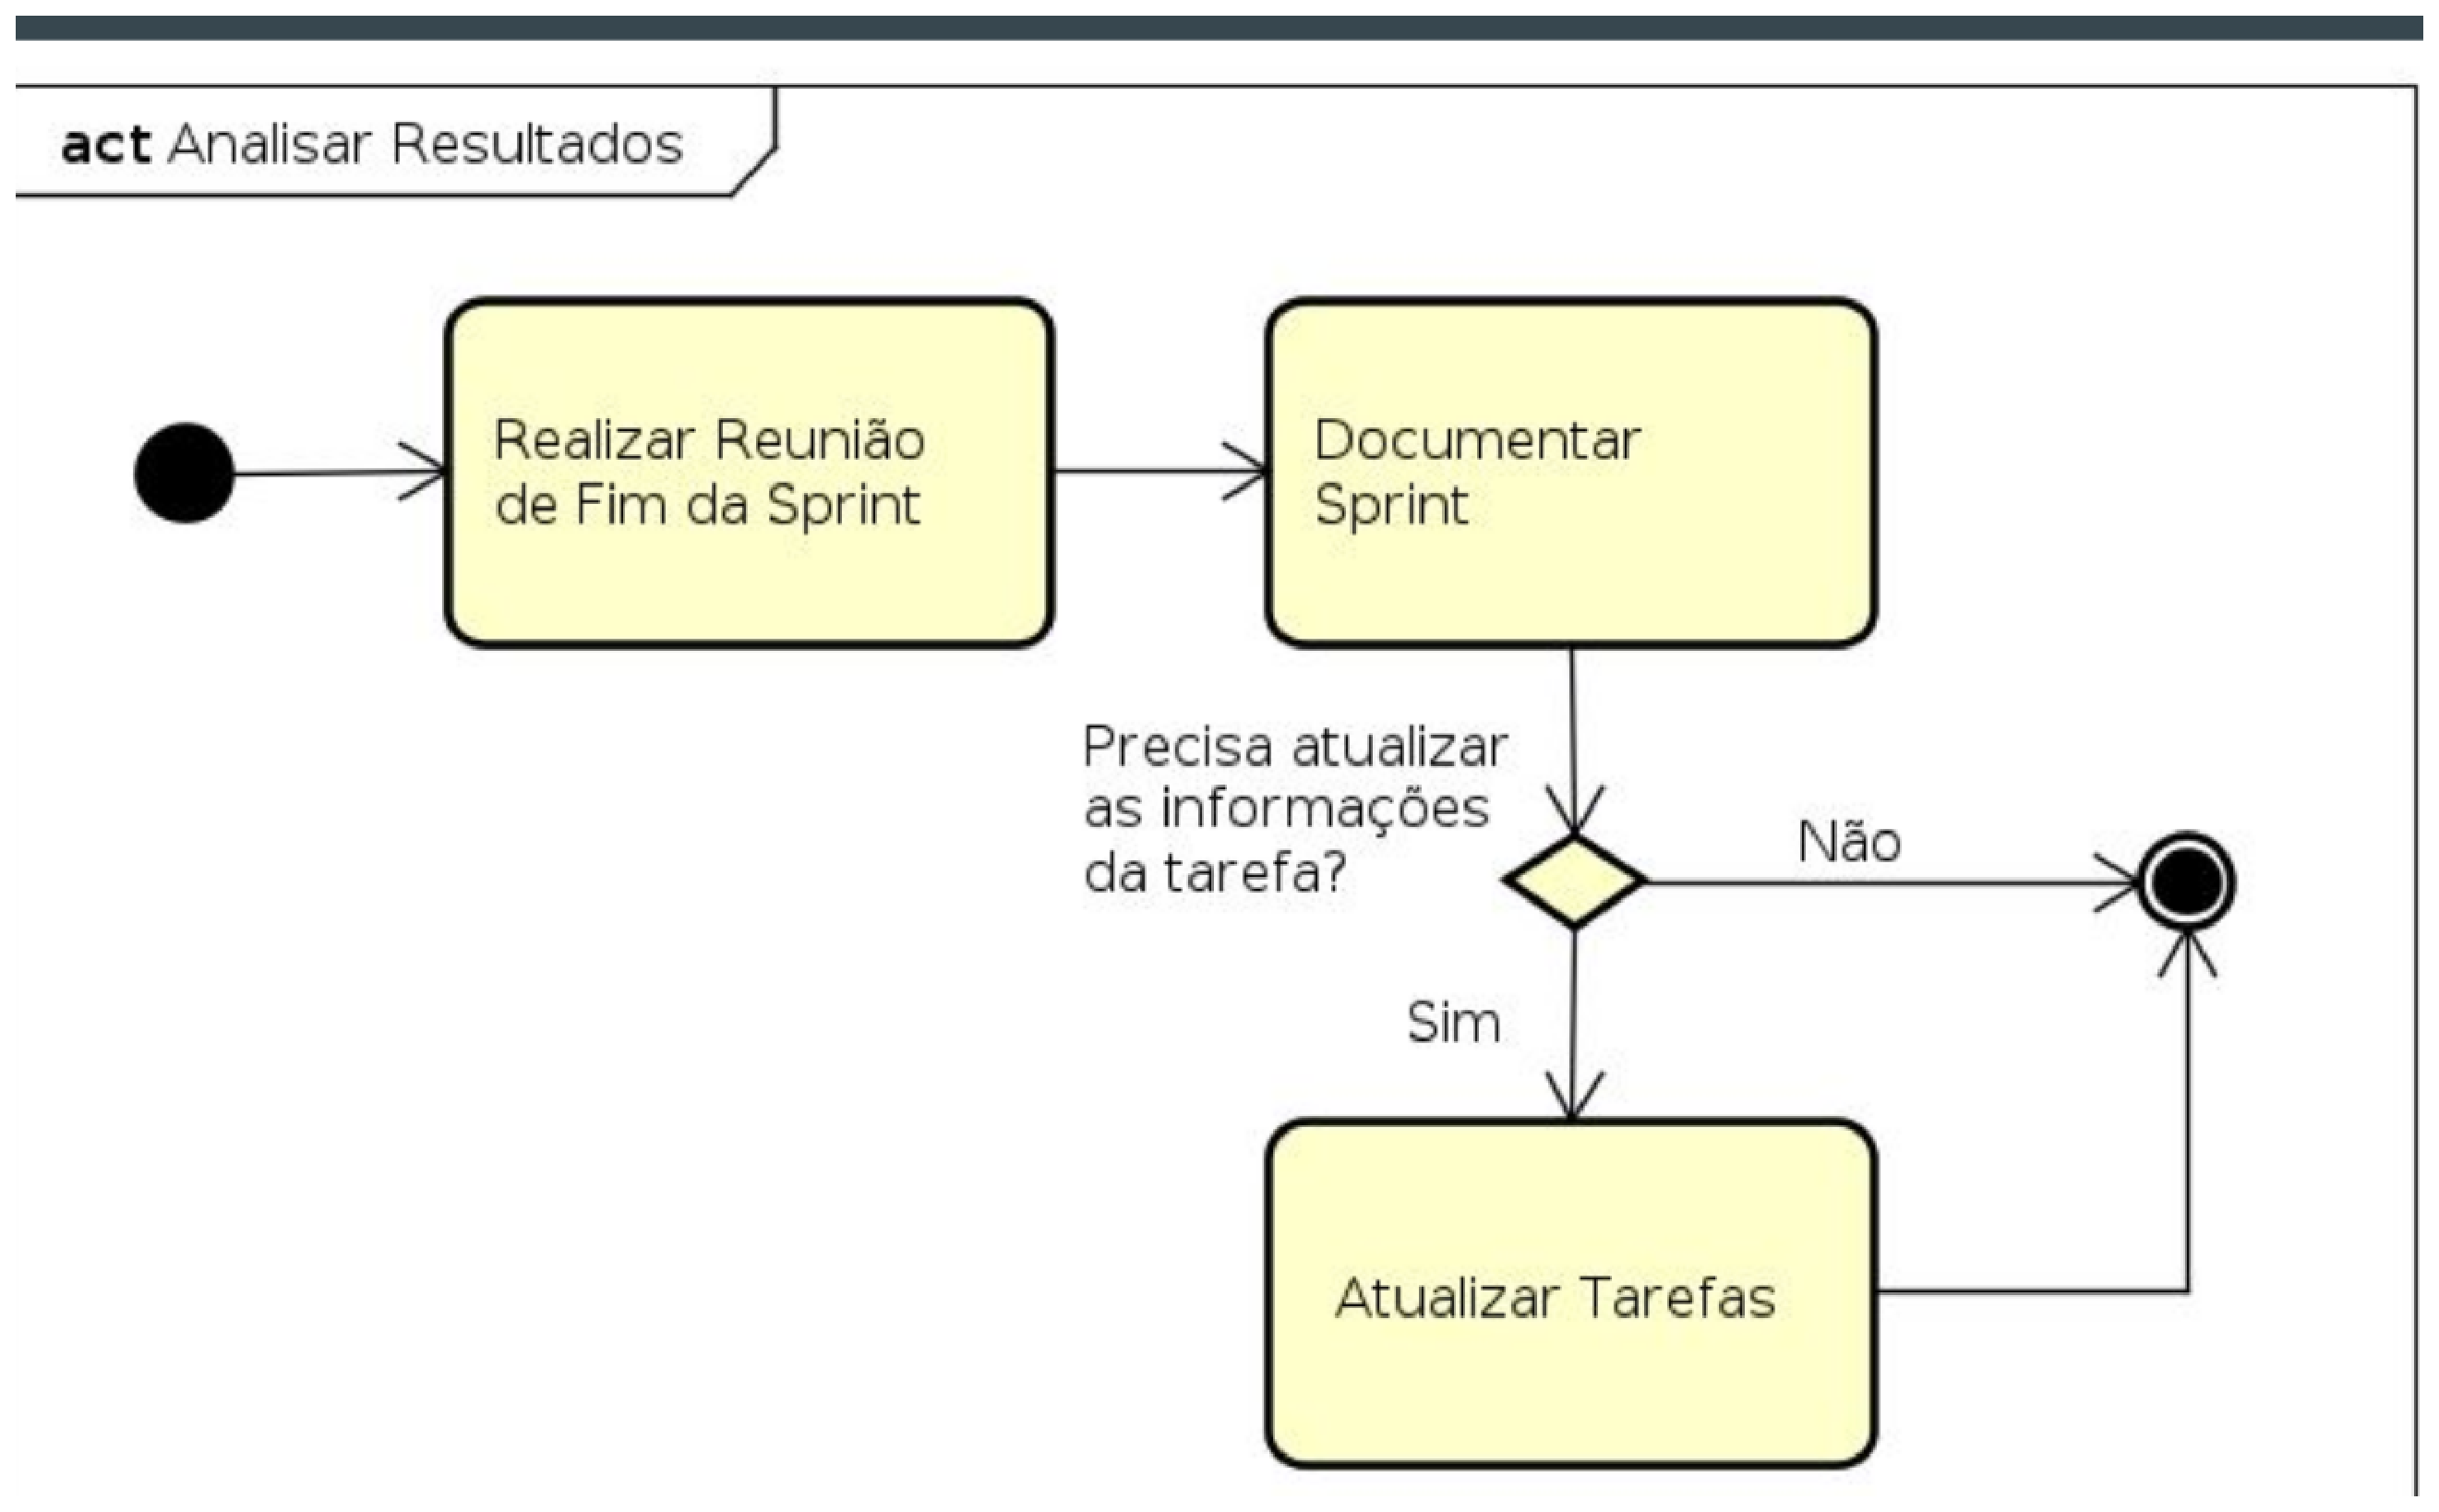
\includegraphics[width=0.9\textwidth]{figuras/processo_mps_resultados.eps}
  \caption{Processo de analisar resultados da sprint para o software Noosfero}
  \label{fig:processo_noosfero_resultado}
\end{figure}

\section*{Análise dos resultados}

\begin{table}[h]
\centering
\resizebox{\textwidth}{!}{\begin{tabular}{|l|l|l|l|l|}
\hline

\rowcolor[HTML]{EFEFEF}
\multicolumn{2}{|c|}{\textbf{Processo Avaliado}} &
\multicolumn{2}{|c|}{} \\ \hline

\rowcolor[HTML]{EFEFEF}
{\textbf{Requerido/Melhoria}} & {\textbf{Resultado Esperado}} &
{\textbf{Problema}} & {\textbf{Sugestão para Corrigir}} \\ \hline

\end{tabular}}
\caption{Relatório de Avaliação}
\label{tab:relatorio_de_avaliacao}
\end{table}

\end{document}
